\documentclass{article}
\usepackage{Estilos/modeloTEEDC}

% Escolha um logo: JOGOS logoludes BMT - logoline
%\edctitle[Imagens/logoline]{Título do Trabalho}
%\edctitle[Imagens/logoludes]{Título do Trabalho}
\edctitle[Imagens/logopesc]{Título do Trabalho}

% Coloque seu nome aqui
\author[$\ddag$]{Nome Aluno}
%\author[$\ddag$]{Geraldo Xexéo}
\affil[$\ddag$]{Programa de Engenharia de Sistemas e Computação \\
COPPE -- Universidade Federal do Rio de Janeiro\\
Brasil}


% Bibliografia deve ser construida com um arquivo 
% no formato BibLaTeX (levemente diferente do BibTeX)
\usepackage[ citestyle=authoryear,articlein=false,
style=ext-authoryear-comp
,natbib=true]{biblatex}
% pode simplesmente trocar o nome do seu arquivo aqui
\addbibresource{bibs/referencias.bib}

\usepackage{hyperref}
\hypersetup{hidelinks,colorlinks = false}

\begin{document}

\maketitle

% seções padrão
\begin{abstract}
    A maioria das publicações usa um resumo não estruturado, que será usado aqui, mas em todo caso, nós usaremos os mesmos tópicos propostos em uma estrutura chamada IMRD~\citep{cmucs}. O artigo, porém, não usará essa estrutura, mas a que aqui está descrita.
    O resumo deve ser construído de forma a fornecer as seguintes informações: 
    \begin{itemize}
        \item introdução, dizendo o que é o artigo
        \item métodos
        \item resultados principais
        \item uma discussão dos resultados, por exemplo, porque é importante
    \end{itemize} 
\end{abstract}

\section{Introdução}

Atualmente, dado o alcance das plataformas de comunicação como Twitter, Facebook, Youtube e afins, disseminar um conhecimento ou uma informação torna-se instantâneo, bastando apenas um clique. Tal fato acaba se tornando um problema que contribui para a disseminação rápida e desenfreada de notícias falsas e outras formas de desinformação. Dado este fato, este trabalho almeja atacar o problema da ``Detecção de \textit{Fake News}'' de modo a avaliar diferentes algorítmos de aprendizado de máquina e técnicas de \textit{NLP - \textit{Natural Language Processing}}. \\

% Com o avanço da tecnologia, torna-se cada vez mais fácil falsificar áudios e vídeos, levando as \textit{fake} news a uma nova e mais preocupante fase conhecida como \emph{Deepfake} que é uma técnica de síntese de imagens humanas baseadas em inteligência  artificial que é usada para sobrepor imagens ou vídeos existentes em outros criando, desta forma, uma informação adulterada que pode ser utilizada em âmbito político, criação de \textit{fakenews}, escandalos pornográficos com celebridades, etc.

O problema gerado pela disseminação de \textit{fake news} se torna mais impactante quando olhamos para temas mais sensíveis como, por exemplo, política ou o mercado financeiro. Nesse contexto a disseminação de notícias falsas pode acarretar diversos problemas. O problema da disceminação desenfreada de notícias falsas deve ser combatido, dado este fato, o Congresso Nacional instalou uma comissão parlamentar mista de inquérito (CPMI)  para apurar a divulgação de informações falsas. \footnote{\url{https://g1.globo.com/politica/noticia/2019/09/04/congresso-instala-comissao-para-investigar-divulgacao-de-informacoes-falsas.ghtml}} Com base neste fato, a utilização de sistemas de identificação de notícias falsas faz-se fundamental para redução da disseminação dessas fontes de desinformação.

% Primeiro parágrafo diz o que o artigo faz.

% Próximos parágrafos fazem uma introdução ao artigo.

\subsection{Motivação}

% Nessa parte deve ser dada uma motivação ao problema, descrevendo porque ele é importante.

% Deve ser indicado um ``gap'' que será investigado, se houver.

As notícias falsas que se espalham pelos meios de comunicação representam uma ameaça real à confiabilidade das informações.
A informação e a detecção de notícias falsas têm atraído cada vez mais atenção nos últimos anos. Notícias falsas
são normalmente escritas intencionalmente para enganar os leitores, o que determina que a detecção de notícias falsas
meramente baseado em conteúdo de notícias é tremendamente desafiador. Enquanto isso, as notícias falsas podem
conter evidências verdadeiras para zombar de notícias verdadeiras e apresentar diferentes graus de falsidade, o que ainda
agrava a dificuldade de detecção \cite{karimi2018}. \\

Segundo \cite{allcot2017}, que fizeram um estudo a respeito da disceminação de \textit{fake news} nas redes sociais durante as eleições presidenciais dos Estados Unidos de 2016, parecem existir duas motivações principais para disseminação de \textit{fake news}. A primeira é pecuniária: artigos de notícias que se tornam virais nas mídias sociais podem atrair anúncios significativos aumentar a receita quando os usuários clicam no site original. 
Esta parece ter sido a principal motivação para a maioria dos produtores cujas identidades foram reveladas. 
A segunda motivação é ideológica pois alguns provedores de notícias falsas procuram promover os candidatos que preferem. \\

Além de impactos sociais e políticos, as \textit{fake news} também podem impactar de forma significativa o mercado financeiro. Prova disso foi o ``Joesley Day'' \footnote{\url{https://www.shsinvestimentos.com.br/artigos-shs/fake-news-e-o-mercado-financeiro-entenda-como-elas-afetam-as-operacoes}} que aconteceu em 2017. Na ocasião, um áudio gravado pelo dono da JBS - que fazia parte de uma delação premiada - registrava o então presidente Michel Temer dando carta branca para comprar o silêncio do ex-deputado Eduardo Cunha, que estava preso por corrupção na operação Lava Jato. Os investidores se desesperaram com a possibilidade de renúncia do presidente e o mercado afundou com os dois pés. O áudio era fake? Não. Só que Joesley sabia o que tinha nas mãos e manipulou o vazamento dele pra ganhar no mercado financeiro através da compra antecipada de dólares. Ele comprou US\$ 3 bilhões e como a moeda disparou, teve um lucro na casa dos US\$ 100 milhões, enquanto muitos investidores agressivos simplesmente quebraram.

\subsection{Objetivo}

% Aqui deve ser dito ou o objetivo, ou as questões de pesquisa ou as hipóteses.

Este trabalho tem como objetivo fazer uma breve revisão da literatura a fim de identificar o estado da arte a respeito do assunto de detecção de notícias falsas, mais específicamente: (i) Quais são as abordagens mais utilizadas em termos de modelagem do problema (Problema de classificação ou regressão); (ii) Quais as técnicas de processamento de linguagem natural e os algoritmos de aprendizado de máquina que são mais eficazes para esta tarefa; (iii) e por fim, executar experimentos utilizando a rede neural \textbf{BERT} e realizar uma comparação com os métodos utilizados na literatura.

% \section{Comentários sobre este modelo}

% O objetivo deste modelo é seguir um padrão para o curso de Tópicos Especiais de Engenharia de Dados e Conhecimento. Ele é baseado na descrição do método científico feita por~\citep[p. 39-40]{Bunge2002}\footnote{Tradução livre do autor}:
% \begin{quote}
% \begin{enumerate}
%     \item Descobrimento do Problema ou lacuna em um conjunto de conhecimentos. Se o problema não está enunciado com clareza, se passa à etapa seguinte, se não, à subsequente;
%     \item Descrição precisa do problema, se possível em termos matemáticos, mas não necessariamente quantitativos, ou uma nova descrição de um velho problema a luz de novos conhecimentos 
%     \item Busca de conhecimentos ou instrumentos relevantes ao problema (por exemplo, dados empíricos, teorias, aparatos de medida, técnica de cálculo ou de medida). Ou seja, inspeção do conhecido para ver se é possível resolver o problema;
%     \item Tentativa de solução do problema com ajuda dos meios identificados. Se essa tentativa falha, passasse à etapa seguinte, se não, à subsequente.
%     \item Invenção de novas ideias (hipóteses, teorias ou técnicas) ou a produção de novos dados empíricos que prometam resolver o problema;
%     \item Obtenção uma solução, exata ou aproximada, do problema com auxílio do instrumental conceitual ou material disponível;
%     \item Por a prova a solução, por exemplo, com ensaios de laboratório ou de campo, e
%     \item Correções necessárias nas hipóteses ou técnicas, ou mesmo na formulação do problema original.
% \end{enumerate}
% \end{quote}

% Essa descrição, ilustrada na Figura \ref{fig:bunge}, é o que se chama na Engenharia de Software de um processo Linear ou em Cascata, mas é óbvio que isso é só uma abstração que facilita a descrição a nível epistemológico. A pesquisa científica é um processo de aprendizado constante, e muitas vezes é necessário, após uma etapa, voltar atrás, ou pular a frente, de forma a melhorar a compreensão do problema, das soluções possíveis, corrigir experimentos, etc.

% \begin{figure}[hbt]
%     \centering
%     \includesvg[width=0.8\textwidth]{Imagens/metodologiabunge}
%     \caption{Metodologia Científica segundo \citet{Bunge2002}, descrita em BPMN~\citep{omg2013bpmn}. Fonte: Do Autor}
%     \label{fig:bunge}
% \end{figure}

% O mesmo autor ainda diz que para que uma ideia seja considerada científica é necessário, mas não suficiente, que ela seja objetivamente testável com dados empíricos~\citep[p. 37]{Bunge2002}. 

% Ainda mais, \citet[p. 40]{Bunge2002} cita \citet{Kuhn1970}, que diz que a melhor forma de aprender a planejar e resolver problemas científicos não é estudar um manual de metodologia, mas estudar e imitar paradigmas ou modelos de investigações que tiveram êxito. \citet{Kuhn2018}, em seu posfácio de 1969, cita outro autor, Michael Polanyi,  defende o conhecimento tácito e diz que ele ``é aprendido fazendo ciência, ao invés de adquirindo regras para fazê-la''~\citep[p. 160]{Kuhn2018}\footnote{O que é um sinal de aviso sobre este texto!}.


% Alguns artigos podem ser tomados como exemplo e não seguem exatamente a estrutura deste modelo. Se você deseja seguir outra estrutura, discuta com o professor primeiro.

% \subsection{Leitura Adicional}

% \begin{itemize}
%     \item Um artigo razoavelmente bem escrito na área de jogos\footnote{\url{https://www.overleaf.com/read/vbhmybkwnmpf}}.
%     \item Não deixem de ler o \citetitle{xexeo2021}.
%     \item Artigos da revista \textit{Pattern Recognition Letters}\footnote{\url{https://www.sciencedirect.com/journal/pattern-recognition-letters}} estão razoavelmente alinhos com padrões de organização aceitos nessa cadeira.
%     \item Alguns alunos devem um trabalho  ainda não publicado ``\textit{Guidelines} para a Construção de uma Dissertação de Mestrado em Computação Aplicada com Problemas de  Mineração de Texto''\footnote{\url{https://www.overleaf.com/read/qpwtkfdssxzr}}.
% \end{itemize}


\section{Revisão}

% Aqui deve conter:
% \begin{itemize}
%     \item uma revisão da teoria necessária para entender o artigo;
%     \item se possível, um histórico das soluções, ou uma taxonomia.\\
% \end{itemize}


Esta seção destina-se a fazer uma breve analise da literatura sobre o tema de \textit{fake news} e tem como objetivo identificar quais são os algoritmos de \textit{machine learning} e técnicas de \textit{NLP} que estão sendo utilizados para atacar esse problema.

Em \citet{parikh2019}, os autores definiram três hipóteses com foco em aprender e entender a origem, disseminação e tom das notícias falsas. Os resultados dessas hipóteses sugerem o seguinte: 1) as notícias falsas não são publicadas em sites populares, mas sim em veículos ou sites menos conhecidos; 2) notícias falsas são mais disseminadas por usuários não verificados do que por usuários verificados; e 3) as notícias falsas são escritas em um tom linguístico específico, embora seja inconclusivo dizer qual (negativo, positivo ou neutro). O resultado da terceira hipotese pode nos fazer indagar sobre se o uso da analise de sentimentos poderia, de alguma forma, nos auxiliar na detecção de \textit{fake news}. Entretanto, em \citet{baarir2020} foi mostrado que utilizar o sentimento presente no texto não auxilia na detecção de \textit{fake news} pois, segundo eles, uma notícia ter um sentimento positivo ou negativo não está relacionado com a veracidade de sua informação. Logo essa simples distincao entre sentimento negativo, positivo ou neutro não é o bastante para a detecção de \textit{fake news}.


Em \citet{DeMagistris2022}, os autores criaram um modelo que utilizava \textit{stance detection} para auxiliar o algoritmo de detecção de \textit{fake news}, O modelo consistia dos seguintes passos: (i) O usuário submetia uma \textit{query} a ser categorizada em uma macro-categoria e baseado no resultado desta classificação o sistema selecionava apenas os artigos relevantes para esse tópico específico; (ii) Uma sub-categoria era assinalada para a \textit{query} com o propósito de reduzir ainda mais o número de doumentos que contribuirão para a avaliação; (iii) O modelo utilizava reconhecimento de entidades nomeadas (\textit{NER}) para filtrar os documentos; (iv) Por fim a \textit{query} era comparada com os documentos relevantes utilizando \textit{embedding} e similaridade de cosenos e os top-k documentos mais similares eram utilizados para \textit{stance classification}. Entretanto os autores descobriram que \textit{stance detection} não ajuda na detecção de \textit{fake news}.

\citet{Wu2021530}, e \citet{Mouratidis20211} combinaram técnicas de \textit{NLP} com \textit{features} oriundas das redes sociais, como por exemplo, \textit{Graph Embedding technique (GEB)} que representa a disseminação da notícia na rede, data da criação da conta do usuário que esta disseminando a notícia, numero de seguidores desse usuário, data do tweet, quantidade de retweets, quantidade de urls presentes no tweet, etc. Esses trabalhos mostraram que \textit{features} oriundas das redes sociais ajudam na detecção de \textit{fake news}.

Em \citet{SelvaBirunda2021406} os autores propuseram uma estrutura de definição de metas para detectar as \textit{fake news} que consistia das seguintes etapas: (i) Para extrair os recursos baseados em texto de nível superior de artigos de notícias genuínos e falsos usando TF-IDF; (ii) Extrair os recursos site\_url de site\_url (domínio); (iii) Estimar uma pontuação de credibilidade de recursos de URL no site baseados em várias fontes e, por fim, (iv) Estimar a credibilidade das notícias integrando os recursos baseados em texto e os Pontuações de Credibilidade. Os autores realizaram experimentos com diversos algoritmos como : SVM, KNN, Naïve Bayes, Logistic Regression, Random Forest, AdaBoost, Decision Tree e, por fim, Gradient Boosting que obteve o melhor resultado com uma acuracia de 99.5%.

\citet{Mouratidis20211} Criaram um modelo de deep learning que utiliza (i) \textit{features} linguísticas como: Quantidade de palavras, Quantidade de sílabas, quantidade media de sílabas, quantidade média de palavras por frase, quantidade de palavras grandes, quantidade de frases longas, quantidade de frases curtas, quantidade de frases na noticia, taxa de advérbios e adjetivos; (ii) Baseado em informações do usuário como: Id do usuário, quantidade de seguidores, número de pessoas que o usuário segue, data da criação da conta, data do tweet, quantidade de likes, quantidade de retweets, Quantiodade de URLs. Segundo os autores, o alto desempenho da detecção de notícias falsas na literatura depende em grande parte da exploração de recursos exclusivamente baseados em contas de usuários ou na exploração de recursos exclusivamente linguísticos. Em contrapartida, esse trabalho dá grande ênfase ao uso de entrada multimodal que varia de incorporação de palavras derivadas automaticamente de texto não estruturado a recursos morfológicos e baseados em string (número de sílabas, número de frases longas, etc.), e de recursos linguísticos de nível superior (como o nível Flesh-Kincaid, a taxa de advérbios-adjetivos etc.).

\citet{Setiawan2021} construíram um \textit{dataset} relacionado ao tema de publicidade e avaliaram o dataset com modelos de aprendizado de maquina e técnicas de \textit{NLP} tais como, TF-IDF, BoW, n-gram (1-GRAM ATE 4-GRAM). Esse trabalho mostrou que o uso de N-grams auxilia no processo de deteccao de \textit{fake news}.
\section{Trabalhos Correlatos}

Aqui o foco nos trabalhos similares e seus resultados.

Deve conter uma tabela que tenha os trabalhos em uma dimensão e as características dos trabalhos em outra dimensão.

O objetivo daqui é estabelecer o estado da arte que o artigo se propõe a melhorar ou indicar novos caminhos.





\section{Proposta}


Este trabalho ataca o problema da detecção de \textit{fake news} binário na língua portuguesa Utilizando a rede Neural BERT. Esta seçâo visa contextualizar alguns tópicos como, por exemplo: Definiçâo do problema; Qual é a base de dados utilizada; Qual o modelo proposto.

% Aqui entram a descrição detalhada do problema sendo tratado e o plano de Solução.

% Aqui será explicada a sua proposta, com cuidado para atingir o objetivo descrito na introdução (ele pode ser lembrado) e como é diferente dos trabalhos correlatos.




\subsection{Definição do problema}

Dado um artigo de notícia $n$, a tarefa de detecção de notícias falsas é prever se essa notícia $n$ é falsa ou verdadeira, isto é,

\begin{center}
    $F(n) =$
    \left\{
    	\begin{array}{ll}
    		0  & \mbox{se } \textit{n é uma notícia falsa} \\
    		1 & \textit{Caso contrário}
    	\end{array}
   
\end{center}

onde $F$ é a função de previsão que queremos aprender.

\subsection{Dataset}

A base de dados utilizada por este trabalho é a \textit{The Fake Br. Corpus}  que foi desenvolvida por \citet{Silva2020}. Esse \textit{dataset} possui um total de 7200 notícias, onde metade dessas notícias é falsa e a outra metade é verdadeira. 

Essa base de dados possui notícias dos seguintes tópicos: economia, ciência e tecnologia, sociedade e notícias diárias, política, religião e, por fim, TV e celebridades. Contudo, vale ressaltar que os tópicos de política, TV e celebridades e sociedade e notícias diárias constituem a maior parte dos dados. A Figura \ref{fig:news_topic_dataset} apresenta como essas notícias se dispersam em cada um desses tópicos. 


\begin{figure}[h]
    \centering
    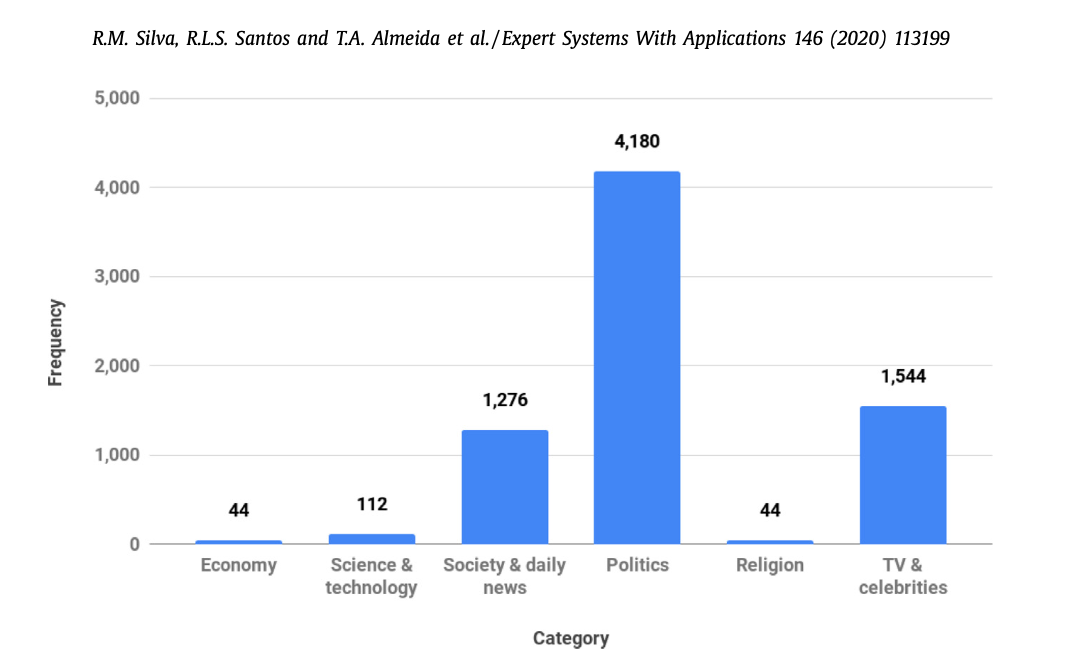
\includegraphics[width=0.85\textwidth]{Imagens/categorias_dataset.png}
    \caption{Frequência das notícias por tópico no Fake Br. Corpus}
    \label{fig:news_topic_dataset}
\end{figure}



\subsection{Modelo Proposto}

O modelo proposto faz uso do \textbf{BERT} (Bidirectional Encoder Representations from Transformers) que é uma técnica para processamento de linguagem natural baseada em \textit{Transformers} que foi desenvolvida pela \textit{Google}. Neste trabalho foi utilizado o Bertimbau (\cite{souza2020bertimbau}) que é um modelo pré-treinado do BERT para o portugês brasileiro. Para este trabalho foi escolhido o Modelo Bertimbau-Base que consiste de 12 camadas de \textit{Transformer encoder}, 12 \textit{attention heads}, 768 \textit{hidden size}, e 110M de parâmetros.\\

O modelo proposto foi construido da seguinte maneira: \\
\begin{enumerate}
    \item Primeiramente, devemos processar o texto de modo a transforma-lo em tokens que deveremos enviar para o classificador;
    \item  Então, extraímos o vetor de \textit{embedding}, de tamanho 768, do token [CLS] provido pelo BERT. (Esse token representa o significado da frase);
    \item A seguir, o utilizamos como \textit{input} para uma camada linear com a função de ativação ReLU;
    \item Por fim temos um vetor de tamanho 2, cada posição desse vetor corresponde a uma categoria dos \textit{labels} (falsa, verdadeira).\\
\end{enumerate}


Toda a implementação do modelo foi realizada em python utilizando a biblioteca pytorch e para o loop de treinamento do modelo foram utilizados o otimizador \textit{Adam} do pytorch com \textit{learning rate} de $1e-5$ e o critério \textit{CrossEntropyLoss} também do pytorch utilizando os parâmetros padrões.

% For a text classification task, we focus our attention on the embedding vector output from the special [CLS] token. This means that we’re going to use the embedding vector of size 768 from [CLS] token as an input for our classifier, which then will output a vector of size the number of classes in our classification task.

% The second variable, which we named pooled_output, contains the embedding vector of [CLS] token. For a text classification task, it is enough to use this embedding as an input for our classifier.

% We then pass the pooled_output variable into a linear layer with ReLU activation function. At the end of the linear layer, we have a vector of size 5, each corresponds to a category of our labels (sport, business, politics, entertainment, and tech).
\section{Experimentos}

\subsection{Configurações do \textit{setup} em que os experimentos foram executados}

Todos experimentos foram realizados em uma máquina com as seguintes configurações: 

\begin{itemize}
    \item Processador: Intel core i9 9900
    \item RAM: 24 GB
    \item Placa de Vídeo: GTX 1660
    \item Python 3.x.x
\end{itemize}

\subsection{Avaliação do modelo}

Durante a execução do experimento o modelo foi treinado por 5 épocas e utilizando a GPU e utilizando apenas o texto da notícia, isto é desconsiderando informções de autor, usuário que propagou, etc. A Base de dados foi dividida da seguinte forma: 80\% dos dados para treinamento do modelo 10\% para a validação que ocorria ao final de cada época de treinamento e 10\% para teste. Foram realizados experimentos utilizando o texto com e sem pré processamento e as métricas utilizadas foram acurácia e F1-Score sobre os resultados obtidos no conjunto de teste.

O pré-processamento utilizado no primeiro experimento foi a remoção de \textit{stop-words}, remoção de acentuação e de pontuação. Para esse primeiro experimento o modelo foi capaz de atingir uma taxa de 93.3\% de acurácia.

Para o segundo experimento, foi utilizado o texto completo da notícia. Vale ressaltar que como o bert aceita no máximo 512 tokens como \textit{input}, o texto pode ser truncado caso o número total de tokens exceda esse valor. Esse experimento conseguiu valores acima de 99\% de acurácia.

A Tabela \ref{table:comparativobert} contrapõe os resultados obtidos pelos experimentos realizados por este artigo e os de \citet{Silva2020} com o propósito de comparar a performance do BERT e dos melhores resultados obtidos sobre esse \textit{dataset}.


\begin{table}
 \label{table:comparativobert}
\begin{tabular}{ |p{3cm}||p{3cm}|p{3cm}|p{3cm}|  }
 \hline
 \multicolumn{4}{|c|}{Tabela Comparativa BERT} \\
 \hline
 Algoritmo & Precision & Recall & F1-Score\\
 \hline
 BERT & X & X & X \\
 SVM & 0.958 & 0.979 & 0.968 \\
 LOGISTIC REGRESSION & 0.964 & 0.976 & 0.971  \\
 \hline
\end{tabular}
\end{table}

% Aqui será descrito como a proposta foi validada.

% Isso implica em escrever como o trabalho foi feito, que dados foram usados (com uma descrição dos dados) e que respostas foram encontradas.


\section{Análise dos Resultados}

% Aqui serão analisados os resultados dos experimentos.

% Os resultados devem ser \textbf{interpretados} e não apenas listados. 

% Deve ser explicado o que os resultados significam para a área.

Como mencionado anteriormente, um dos objetivos deste trabalho é identificar as abordagens mais utilizadas para atacar o problema da detecção de \textit{fake news}. Com base na revisão da literatura feita por este trabalho, podemos citar como um dos resultados os seguintes achados:
\begin{itemize}
\item  As técnicas  de \textit{NLP} que se mostraram mais eficazes foram \textit{BoW, TF-IDF e N-GRAM} e os algoritmos que se sobressaíram foram \textit{SVM, LR} e algoritmos baseados em redes neurais ou \textit{Deep Learning}, principalmente os que consideram informações do usuário para a detecção de \textit{fake news};  
\item O sentimento da presente no conteúdo da notícia não auxilia na detecção de \textit{fake news}, pois como foi mostrado em \citep{baarir2020} o sentimento da notícia não influencia em sua veracidade; 
\item A utilização de \textit{Stance Detection} também não ajuda na detecção de \textit{fake news} como mostrado em \citep{DeMagistris2022}.
\end{itemize}

Outro resultado deste trabalho foi a obtenção de uma taxa de acerto de 99\% na detecção de \textit{fake news} utilizando o \textit{Google BERT} no segundo experimento, que foi superior ao do primeiro experimento,que obteve cerca de 93\% de acerto, que também utilizava o \textit{BERT} porém fazendo uso pré-processamento do texto. Esse resultado mostra que o \textit{Google BERT} funciona melhor utilizando o texto em linguagem natural. Também vale ressaltar que, nesses experimentos, não foram utilizadas informações a respeito do autor da notícia ou do usuário que a propagou oque indica que apenas o texto da notícia, para a base de dados utilizada, foi suficiente para a distinção entre notícias falsas e verdadeiras. 

   
\input{Secoes/07conclusão.tex}

\nocite{*}
\printbibliography

\end{document}
